\pgfdeclarelayer{last}
\pgfdeclarelayer{background}
\pgfsetlayers{last,background,main}

\def\sourcesink{{(0,0)/s}, {(3, 1)/t}}
\def\network{{(0.5,0.5)/c}, {(1,1)/d}, {(0.5, 2.5)/e}, {(1.25, 2.5)/f}, {(1.25, 1.5)/g}, {(1.25, 0.5 )/h}, {(1.75, 0.5)/i}, {(1.80, 1.8)/j}, {(1.20, -1)/k}, {(1.40, -0.6)/l}, {(2.6, 0.7)/m}, {(1.8, 0)/-}}
\def\connect{s/c, c/d, d/h, h/i, i/-, -/l, l/k, d/g, g/j, j/f, f/e, i/m, m/t}

\colorlet{circle edge}{black!50}
\colorlet{circle area}{gray!20}

\tikzset{
  filled/.style={fill=circle area, thick},
  outline/.style={draw=circle edge, thick}
  }

\setlength{\parskip}{5mm}

\tikzstyle{edge} = [draw, thick, -]
\tikzstyle{vertex}=[circle,fill=black!25,minimum size=10pt,inner sep=0pt]
\tikzstyle{invis-vertex}=[circle,fill=white!100,minimum size=0pt, inner sep=0pt]
\tikzstyle{edgeBackground} = [draw, line width=2cm,-,gray!20] 
\tikzstyle{real edge} = [draw, line width=8pt,-, gray!70]

\subfloat[Linear Swept Sphere]{\label{fig:rdr1}
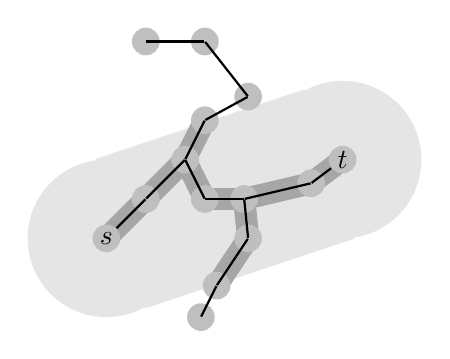
\begin{tikzpicture}  

  % Definition of the radii
  \def\firstradius{(0,0) circle (1cm)};
  \def\secondradius{(3, 1) circle (1cm)};

  \begin{pgfonlayer}{last}
    \fill[filled] \firstradius;
    \fill[filled] \secondradius;
  \end{pgfonlayer}

  % The real source and sink
  \foreach \pos/\name in \sourcesink {
    \node[invis-vertex] (\name-) at \pos {};
    \node[vertex] (\name) at \pos {$\name$};
  }

  \begin{pgfonlayer}{last}   
    \path[edgeBackground] (s) -- (t);
  \end{pgfonlayer}

  % the extra nodes
  \foreach \pos/\name in \network {
    \node[invis-vertex] (\name) at \pos {}; 
    \node[vertex] () at \pos {};
  }

  % The connections between them
  \begin{pgfonlayer}{background}
  \foreach \source/\sink in {s-/c, c/d, d/h, h/i, i/m, m/t-, i/-, -/l, d/g}
    \path[real edge] (\source) -- (\sink);
  \end{pgfonlayer}

  % The nodes they can reach
  \foreach \source/\sink in \connect
    \path[edge] (\source) -- (\sink);

\end{tikzpicture}}
% Remove empty line
\subfloat[Circle]{\label{fig:rdr2}
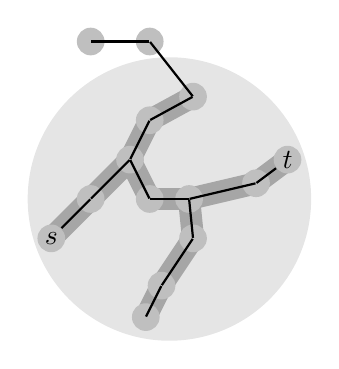
\begin{tikzpicture}  

  % Definition of the radii
  \def\radius{(1.5,0.5) circle (1.8)};
  \begin{pgfonlayer}{last}
    \fill[filled] \radius;
  \end{pgfonlayer}

  % The real source and sink
  \foreach \pos/\name in \sourcesink {   
    \node[invis-vertex] (\name-) at \pos {};
    \node[vertex] (\name) at \pos {$\name$};
  }
   
  % the extra nodes
  \foreach \pos/\name in \network {
    \node[invis-vertex] (\name) at \pos {}; 
    \node[vertex] () at \pos {};
  }

  % The connections between them
  \begin{pgfonlayer}{background}
    \foreach \source/\sink in {s-/c, c/d, d/h, h/i, i/m, m/t-, i/-, -/l, d/g, g/j, l/k}
    \path[real edge] (\source) -- (\sink);
  \end{pgfonlayer}

  % The nodes they can reach
  \foreach \source/\sink in \connect
    \path[edge] (\source) -- (\sink);
\end{tikzpicture}}
% Remove empty line
\subfloat[Rectangle]{\label{fig:rdr3}
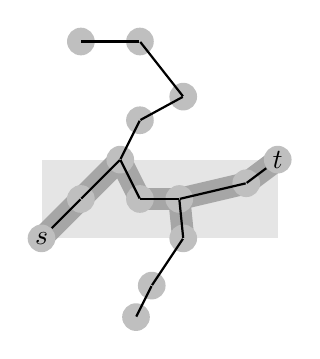
\begin{tikzpicture}  

  % Definition of the radii
  \def\rectangle{(0,0) rectangle (3,1)};
  \begin{pgfonlayer}{last}
    \fill[filled] \rectangle;
  \end{pgfonlayer}      

  % The real source and sink
  \foreach \pos/\name in \sourcesink {  
    \node[invis-vertex] (\name-) at \pos {};
    \node[vertex] (\name) at \pos {$\name$};
  }
  % the extra nodes
  \foreach \pos/\name in \network {   
    \node[invis-vertex] (\name) at \pos {};
    \node[vertex] () at \pos {};
  }  

  % The connections between them
  \begin{pgfonlayer}{background}
    \foreach \source/\sink in {s-/c, c/d, d/h, h/i, i/-, i/m, m/t-}
      \path[real edge] (\source) -- (\sink);
  \end{pgfonlayer}

  % The nodes they can reach
  \foreach \source/\sink in \connect
    \path[edge] (\source) -- (\sink);
\end{tikzpicture}}
